\section{Serielle Schnittstelle}

\begin{defi}{Parallele Schnittstelle}
    \emph{Parallele Schnittstellen} übertragen Bits \emph{parallel} über mehrere, parallele Leitungen.
\end{defi}

\begin{defi}{Serielle Schnittstelle}
    \emph{Serielle Schnittstellen} übertragen Bits nacheinander auf einer Leitung.

    In der Praxis zeigt sich, dass serielle Schnittstellen schneller sind, da sie keine Probleme wie Laufzeit der Signale, \enquote{übersprechen} oder Leitungskapazitäten haben.
\end{defi}

\begin{defi}
    Schnittstellen werden genutzt, um zwischen einem Mikrocontroller und Sensoren oder einem Host System zu kommunizieren.

    Eigenschaften:
    \begin{itemize}
        \item \emph{Physikalische Schnittstelle}:
              \begin{itemize}
                  \item Spannungspegel
                  \item Anzahl der Kanäle
              \end{itemize}
        \item \emph{Arbeitsweise}:
              \begin{itemize}
                  \item \emph{Synchron} (mit Taktsignal)
                  \item \emph{Asynchron} (ohne Taktsignal)
              \end{itemize}
        \item \emph{Kommunikationsrichtung}:
              \begin{itemize}
                  \item \emph{simplex}: Ausschließlich eine Richtung
                  \item \emph{halb-duplex}: Abwechselnd in eine Richtung
                  \item \emph{voll-duplex}: zeitgleich in beide Richtungen
              \end{itemize}
        \item \emph{Flussteuerung}
        \item \emph{Topologie}:
              \begin{itemize}
                  \item Punkt-zu-Punkt
                  \item Bus
              \end{itemize}
    \end{itemize}
\end{defi}

\begin{defi}{Schrittgeschwindigkeit}
    [Bd] = $\frac{1}{t}$ = Baud
\end{defi}

\subsection{UART und SPI}

\begin{defi}{UART}
    \emph{Universal Asynchronous Receiver/Transmitter (UART)} ist eine asynchrone Punkt-zu-Punkt, die grundsätzlich voll-duplex Betrieb erlaubt.

    Im einfachsten Fall existieren nur 2 Leitungen, die über Kreuz zwischen zwei Geräten angeschlossen werden:
    \begin{itemize}
        \item \texttt{TX} (Senden)
        \item \texttt{RX} (Empfangen)
    \end{itemize}

    Zu Beginn der Kommunikation muss man sich auf folgende Einstellungen einigen:
    \begin{itemize}
        \item 7 oder 8 Datenbits
        \item Paritätsbit 1 wenn Anzahl 1en gerade oder ungerade.
        \item 1 oder 2 Stopbits
    \end{itemize}

    Mit UART lassen sich z. B. 150m bei 9600 Baud überbrücken.

    Die UART Schnittstelle verwendet manchmal spezielle Leitungen zur Datenflusssteuerung zwischen dem \emph{Data Communication Equipment (DCE)} und dem \emph{Data Terminal Equipment (DTE)}:
    \begin{itemize}
        \item \emph{Ready To Send (RTS)}
        \item \emph{Clear To Send (CTS)}
        \item \emph{Data Terminal Ready (DTR)}
        \item \emph{Data Set Read (DSR)}
    \end{itemize}

    In der Praxis werden diese Leitungen jedoch nicht verwendet, sondern die Flussteuerung z. B. per Software realisiert.
    Daher sieht man auf dem Launchpad auch nur \texttt{RX} und \texttt{TX}
\end{defi}

\begin{defi}{eUSCI}
    \emph{Enhanced Universal Serial Communication Interface} Einheiten können im \emph{UART} Modus betrieben werden.

    \texttt{eUSCI\_A0} ist normalerweise über zwei Jumper an das Backchannel-UART angeschlossen.
\end{defi}

\begin{bonus}{Empfangen einer Nachricht}
    Zum Empfangen benötigen wir verschiedene Register.

    Zu Beginn wird die Nachricht in das \emph{Receive Shift Register} aufgenommen.

    Dieses leitet die empfangenen Daten in den \emph{Receive Buffer} weiter.
    Der Buffer nimmt nur Daten an, wenn er leer ist.

    Dabei können verschiedene Fehler auftreten:
    \begin{itemize}
        \item \emph{Break (BRK)} wird gesetzt, wenn das Empfangssignal länger als die Dauer eines Datenrahmens auf logisch 0 liegt.
        \item \emph{Overrun Error (OE)} wird gesetzt, wenn \texttt{UCSxRXBUF} bereits gefüllt ist, und ein komplettes neues Datenwort Shift-Register eingegangen ist.
    \end{itemize}
\end{bonus}

\begin{defi}{SPI}
    Ein \emph{Serial Peripheral Interface (SPI)} ist ein synchrones voll-duplex Bussystem mit einer 1:N Topologie.

    Es gibt u. a. folgende variable Größen:
    \begin{itemize}
        \item Wortlänge
        \item LSB bzw MSB first
        \item Taktflanke
        \item Frequenz
    \end{itemize}

    Dazu werden 4 Signale genutzt:
    \begin{itemize}
        \item \emph{Serial CLocK (SCLK)}, gesetzt von Main
        \item \emph{Main Out, Sub In (MOSI)}
        \item \emph{Main In, Sub Out (MISO)}
        \item \emph{Sub Select (/SS)}
    \end{itemize}

    Jedes Subsystem hat ein eigenes \emph{Sub Select}-Signal.
    Alle anderen Leitungen werden gemeinsam genutzt.

    \emph{/SS} ist \texttt{LOW}-Aktiv, d. h. eine logische 0 selektiert den Sub.
\end{defi}

\subsection{I2C}

\begin{defi}{I2C}
    \emph{Inter-Integrated Curcuit (I2C)} ist ein populäres Bussystem zur Anbindung von integrierten Schaltungen.

    Es ist eine synchrone, halb-duplex Schnittstelle mit einer 1:N Topologie.

    Es werden lediglich zwei Leitungen genutzt:
    \begin{itemize}
        \item \emph{Serial CLock (SCL)}
        \item \emph{Serial DAta (SDA)}
    \end{itemize}

    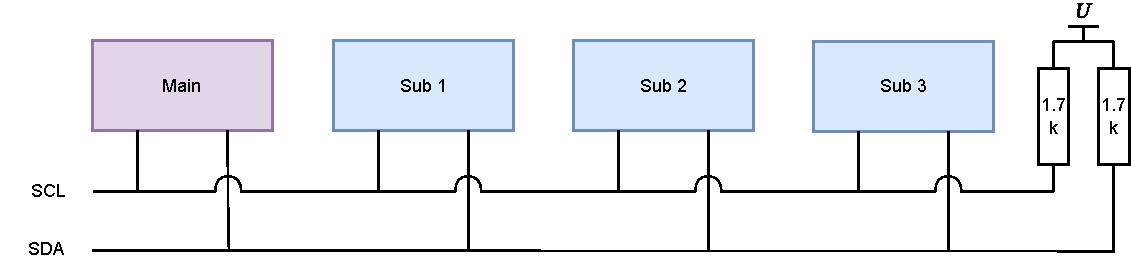
\includegraphics[width=\textwidth]{includes/figures/defi_i2c.pdf}
\end{defi}

\begin{bonus}{Besonderheiten I2C}
    \begin{itemize}
        \item Main/Sub Architektur wie bei SPI
        \item Main initiiert die Kommunikation
        \item Nur eine Datenleiten, trotzdem Datenaustausch in beide Richtungen möglich
        \item Auch die Taktleitung kann von beiden Kommunikationspartnern genutzt werden.
    \end{itemize}
\end{bonus}

\begin{defi}{Open Drain}
    Wenn ein Kommunikationspartner eine Leitung auf \texttt{HIGH} und ein anderer auf \texttt{LOW} setzt, kann es zu einem Kurzschluss kommen.
    Um dem entgegenzuwirken wurden \emph{Open-Drain Ausgangsstufen} implementiert:

    \begin{center}
        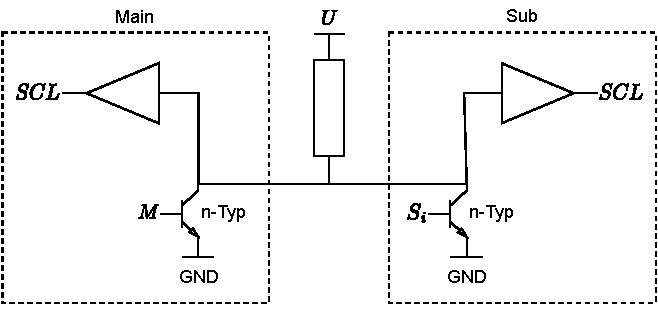
\includegraphics[width=0.5\textwidth]{includes/figures/defi_open_drain.pdf}
    \end{center}

    Der Ruhezustand ist \texttt{HIGH}.
    Wenn ein Gerät die Leitung selber nicht auf \texttt{LOW} zieht, kann es den Wert einer Leitung auslesen.
\end{defi}

\begin{bonus}{Taktraten}
    Die Pullup-Widerstände müssen richtig dimensioniert werden, damit die Pegelwechsel auf den Leitungen schnell genug passieren.

    I2C arbeitet durch die Open-Drain Ausgänge langsamer als SPI.
    Üblich sind Taktraten von 100kHz bus 1MHz.

    Im Gegensatz zu SPI werden bei I2C immer 8 Bit und ein \texttt{ACK}-bit versendet, die entweder als Geräteadresse oder Daten interpretiert werden.
\end{bonus}

\begin{defi}{Datenaustausch}
    Jede Datenübertragung wird von einer sogenannten \texttt{START}- und \texttt{STOP}-Bedingung eingerahmt.

    Bei \texttt{START} wird zuerst \emph{SDA}, dann \emph{SCL} auf \texttt{LOW} gesetzt.
    Bei \texttt{STOP} wird zuerst \emph{SCL}, dann \emph{SDA} auf \texttt{HIGH} gesetzt.

    Nach der \texttt{START}-Bedingung erfolgt die Übertragung von 8 bit, wobei \texttt{SDA} nur seinen Pegel ändern darf, wenn \texttt{SCL} \texttt{LOW} ist.

    Der Wert von \texttt{SDA} wird übernommen, wenn \texttt{SCL} \texttt{LOW} ist.

    Beim \texttt{ACK} lässt der Main die \texttt{SDA}-Leitung lost, d. h. sie wäre normalerweise auf \texttt{HIGH}.
    Das angesprochene Sub-System muss die Leitung auf \texttt{LOW} setzten, damit das Main-System weiß, dass das Paket empfangenen wurde.

    Der Empfänger kann nach dem \texttt{ACK} die Leitung auf \texttt{LOW} lassen, damit der Sender langsamer sendet.
\end{defi}

\begin{defi}{Adressierung}
    Jedes I2C-Gerät wird über eine 7 bit Adresse adressiert.
    Ein weiteres bit ($R / \bar{W}$) gibt an, ober das Main.System die Daten schreiben oder Lesen möchte.

    Beim \emph{lesenden} Zugriff wird zunächst auch die Adresse des I2C-Geräts und die Adresse des Registers vom Main-System gesendet.
    Danach wird eine weitere \texttt{START}-Bedingung gesendet und nach dem Schreiben der Register-Adresse übernimmt das Sub-System die \texttt{SDA}-Leitung und versendet die Daten.

    Das Main-System signalisiert mit einem \texttt{NACK}, dass er keine weiteren Daten empfangenen möchte.
\end{defi}

\begin{bonus}{Empfangen einer Nachricht}
    Zum Empfangen benötigen wir verschiedene Register.

    Zu Beginn wird die Nachricht in das \emph{Receive Shift Register} aufgenommen.

    Dieses leitet die empfangenen Daten in den \emph{Receive Buffer} weiter.
    Der Buffer nimmt nur Daten an, wenn er leer ist.
\end{bonus}

\begin{bonus}{Senden einer Nachricht}
    Zum Senden einer Nachricht schreiben wir die Daten in  den \emph{Transmit Buffer}.

    Zu Beginn wird die Nachricht in des \emph{Transmit Shift Register} aufgenommen.
    Die Sub-Adresse befindet sich in einem eigenen Register.

    Solange Daten im \texttt{Transmit Buffer} liegen, wird das \emph{Transmit Shift Register} gefüllt.
\end{bonus}